%!TeX root = ../main.tex

% ==========================================
% CHAPTER 2: KINEMATIC AND PROBABILISTIC MODELS 
% ==========================================
\chapter{Kinematic and Probabilistic Models of Mobile Robots}
\label{Ch:Kinematic}
This chapter establishes the mathematical and theoretical foundations governing the locomotion of the analyzed robotic platforms. Before addressing the software configuration of the navigation stack, it is essential to formally define the physical constraints that dictate how the robot interacts with its environment. The chapter begins by defining the configuration space and the fundamental distinction between holonomic and non-holonomic constraints (Section~\ref{sec:intro_kin}). Subsequently, it derives the direct and inverse kinematics for both the differential drive PMB2 (Section~\ref{sec:diff_model}) and the omnidirectional OmniBase (Section~\ref{sec:omni_model}). Finally, acknowledging that real-world locomotion is inevitably affected by unmodeled physical interactions, Section~\ref{sec:probabilistic_motion_models} introduces the probabilistic motion models, characterizing the distinct odometric noise profiles of both drives. These theoretical principles provide the necessary justification for the infrastructural adaptations and algorithmic tuning detailed in Chapter~\ref{ch:architecture}.

\section{Introduction to Mobile Robot Mobility}
\label{sec:intro_kin}

The study of mobile robot kinematics deals with the mathematical description of motion without considering the forces that cause it. Before analyzing the specific models of the TIAGo robot, it is essential to define the basic concepts of mobility, configuration space, and kinematic constraints.

For a mobile robot operating in a 2D planar environment, its pose (or posture) is uniquely defined by a vector in the configuration space. Typically, this vector is denoted as:
\begin{equation}
    q = \begin{bmatrix} x \\ y \\ \theta \end{bmatrix} \in \mathbb{R}^2 \times S^1
\end{equation}
where $x$ and $y$ represent the Cartesian coordinates of a reference point on the robot chassis, and $\theta$ represents its orientation (heading) with respect to a global reference frame \cite{palli_amr_slides}.

The mobility of a robot is strictly determined by the mechanical design of its wheels and how they interact with the ground. Assuming the ideal condition of pure rolling without slipping, each wheel imposes specific kinematic constraints on the robot's motion. In mobile robotics, we generally distinguish between two main categories of constraints:

\begin{itemize}
    \item \textbf{Holonomic constraints:} These are constraints on the position (or configuration) variables. A robot is considered holonomic if its controllable degrees of freedom (DOFs) are equal to the total degrees of freedom of its configuration space. In a planar environment, a holonomic robot can instantaneously move in any direction $(x, y)$ while independently changing its orientation $\theta$.
    
    \item \textbf{Non-holonomic constraints:} These are differential constraints on the robot's velocities that cannot be integrated into finite position constraints. They limit the instantaneous directions in which the robot can move, but they do not reduce the overall reachable configuration space. A classic example is a standard car, which can be parked anywhere but cannot instantaneously move sideways.
\end{itemize}

The two bases of the TIAGo robot analyzed in this thesis perfectly represent these two opposite categories: the standard PMB2 base is a non-holonomic system, whereas the OmniBase is a fully holonomic system. The following sections will mathematically detail the kinematic implications of these designs.


\section{Differential Drive Model (TIAGo PMB2)}
\label{sec:diff_model}

The default mobile base of the TIAGo robot is the PMB2 (PAL Mobile Base 2), which employs a differential drive locomotion system \cite{pal_tiago_base}. According to the manufacturer, this configuration provides high agility in standard indoor environments with a circular footprint, making it ideal for general-purpose navigation tasks \cite{pal_blog_omni_diff}. The configuration consists of two independently actuated, coaxial wheels located at the sides of the robot, supplemented by four passive caster wheels for mechanical stability.

\subsection{Physical Configuration}

Let us define the geometric parameters of the PMB2 base (Figure~\ref{fig:diff_drive_model}):
\begin{itemize}
    \item $r$: radius of the driven wheels;
    \item $d$: wheelbase, defined as the distance between the centers of the two driven wheels;
    \item $\omega_R, \omega_L$: angular velocities of the right and left wheel, respectively.
\end{itemize}

% --- INIZIO INSERIMENTO IMMAGINE ---
    \begin{figure}[htbp]
        \centering
        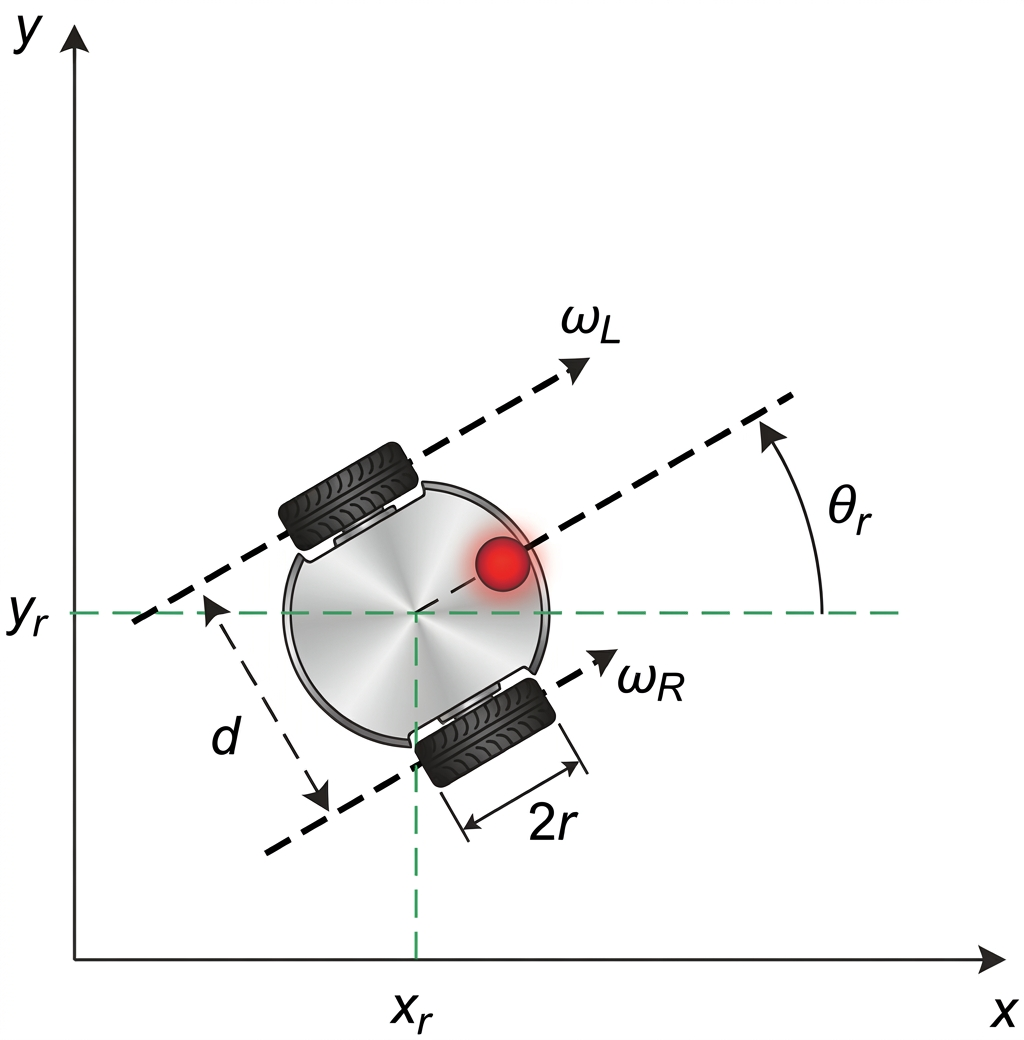
\includegraphics[width=0.5\textwidth]{images/Ch2/Modello unicycle robot.jpg}
        \caption{Kinematic model of a differential drive robot (Image adapted from \cite{palli_amr_slides}).}
        \label{fig:diff_drive_model}
    \end{figure}
% --- FINE INSERIMENTO IMMAGINE ---

\subsection{Direct and Inverse Kinematics}

Because the differential drive is kinematically equivalent to a single steerable wheel located at the midpoint of the wheel axle (the red circle), it can be mathematically described by the \emph{unicycle kinematic model} \cite{palli_amr_slides}.

By controlling the angular velocities of the two independent wheels, it is possible to govern both the translational velocity $v$ and the rotational velocity $\omega$ of the robot. The \emph{Direct Kinematics} equations mapping the individual wheel velocities to the robot's local velocities are:
\begin{equation}
    v = \frac{r}{2} (\omega_R + \omega_L) \quad\quad, \quad \quad \omega = \frac{r}{d} (\omega_R - \omega_L)
\end{equation}

In autonomous navigation frameworks like ROS 2, the navigation stack generates global velocity commands. Therefore, the robot controller must compute the \emph{Inverse Kinematics} to translate the desired $[v, \omega]^T$ into the required wheel speeds:
\begin{equation}
    \omega_R = \frac{v + \frac{\omega d}{2}}{r}, \quad \quad \omega_L = \frac{v - \frac{\omega d}{2}}{r}
\end{equation}

The state space equations governing the robot's global pose $q = [x, y, \theta]^T$ are given by the following matrix formulation \cite{palli_amr_slides}:
\begin{equation}
    \dot{q} = \begin{bmatrix} \dot{x} \\ \dot{y} \\ \dot{\theta} \end{bmatrix} =
    \begin{bmatrix} \cos\theta & 0 \\ \sin \theta & 0 \\ 0 & 1 \end{bmatrix}
    \begin{bmatrix} v \\ \omega \end{bmatrix} =     
    \begin{bmatrix} 
    \frac{r\cos \theta}{2} & \frac{r\cos \theta}{2} \\ 
    \frac{r\sin \theta}{2} & \frac{r\sin \theta}{2} \\ 
    \frac{r}{d} & -\frac{r}{d} 
    \end{bmatrix}
    \begin{bmatrix} \omega_R \\ \omega_L \end{bmatrix}
\end{equation}
where $\dot{x}$ and $\dot{y}$ are the linear velocities along the global axes, and $\dot{\theta}$ is the angular velocity of the robot.

\subsection{Non-Holonomic Constraints and Mobility}
\label{subsec:non holonomic constr}

The differential drive imposes a strict limitation on the robot's mobility: the wheels are assumed to be subject to the conditions of pure rolling and no lateral slipping. As a consequence, the robot cannot translate instantaneously along the axis collinear with the wheel axle.

Mathematically, the velocity in the lateral local direction must always be zero. This physical limitation is expressed by the following non-holonomic mobility constraint:
\begin{equation}
    \dot{x} \sin\theta - \dot{y} \cos\theta = 0.
\end{equation}

Following a formal approach, this constraint can be rewritten in the \emph{Pfaffian form} \\ $A(q)\dot{q} = 0$ \cite{palli_amr_slides}:
\begin{equation}
    \begin{bmatrix} \sin \theta & -\cos \theta & 0 \end{bmatrix}
    \begin{bmatrix} \dot{x} \\ \dot{y} \\ \dot{\theta} \end{bmatrix} = 0
\end{equation}

where $A(q)$ is the constraint. Because this differential equation cannot be integrated to yield a finite constraint on the position variables $x$ and $y$, the system is strictly non-holonomic. This entails that while the PMB2 can eventually reach any point and orientation in its operational 2D space, it must execute complex, multi-step maneuvers (e.g., rotate in place, then move forward) to perform lateral displacements. As will be demonstrated in the experimental chapters, and highlighted by PAL Robotics \cite{pal_blog_omni_diff}, this heavily influences path planning strategies and increases the control effort required in narrow spaces.


% ---------------------------------------------------------
\section{Omnidirectional Drive Model (TIAGo OmniBase)}
\label{sec:omni_model}

To overcome the maneuverability limitations of non-holonomic platforms, the TIAGo robot can be equipped with the OmniBase. As stated by the manufacturer, this platform provides a fully holonomic locomotion system, granting 360-degree mobility \cite{pal_tiago_omnibase}. This allows the robot to perform instantaneous translations in any direction while independently changing its orientation, an essential feature for precision positioning and navigation in highly complex and dynamic environments \cite{pal_blog_omni_diff}.

\subsection{Physical Configuration}

The TIAGo OmniBase is equipped with four Swedish wheels, specifically of the \emph{Mecanum} type. As highlighted by Yepez-Figueroa et al. \cite{yepez-figueroa_design_2025}, while standard omnidirectional wheels feature passive rollers mounted at $90^\circ$ relative to the main wheel axis, Mecanum wheels have passive rollers oriented at an angle of $\alpha = 45^\circ$. 

This specific design allows the four wheels to be mounted strictly parallel to the robot's longitudinal axis ($x$-axis), providing a stable rectangular footprint while still enabling full planar mobility \cite{yepez-figueroa_design_2025}. Let us define the geometric parameters of the OmniBase (Figure~\ref{fig:mecanum_model}):
\begin{itemize}
    \item $r$: radius of the Mecanum wheels;
    \item $a$: longitudinal distance from the robot's geometric center to the wheel axles along the $u_f$-axis (the robot's local forward axis);
    \item $b$: lateral distance from the robot's geometric center to the wheels along the $u_l$-axis (the robot's local lateral axis);
    \item $\omega_{FL}, \omega_{FR}, \omega_{RL}, \omega_{RR}$: angular velocities of the Front-Left, Front-Right, Rear-Left, and Rear-Right wheels, respectively.
\end{itemize}

% --- INIZIO INSERIMENTO IMMAGINE ---
\begin{figure}[htbp]
    \centering
    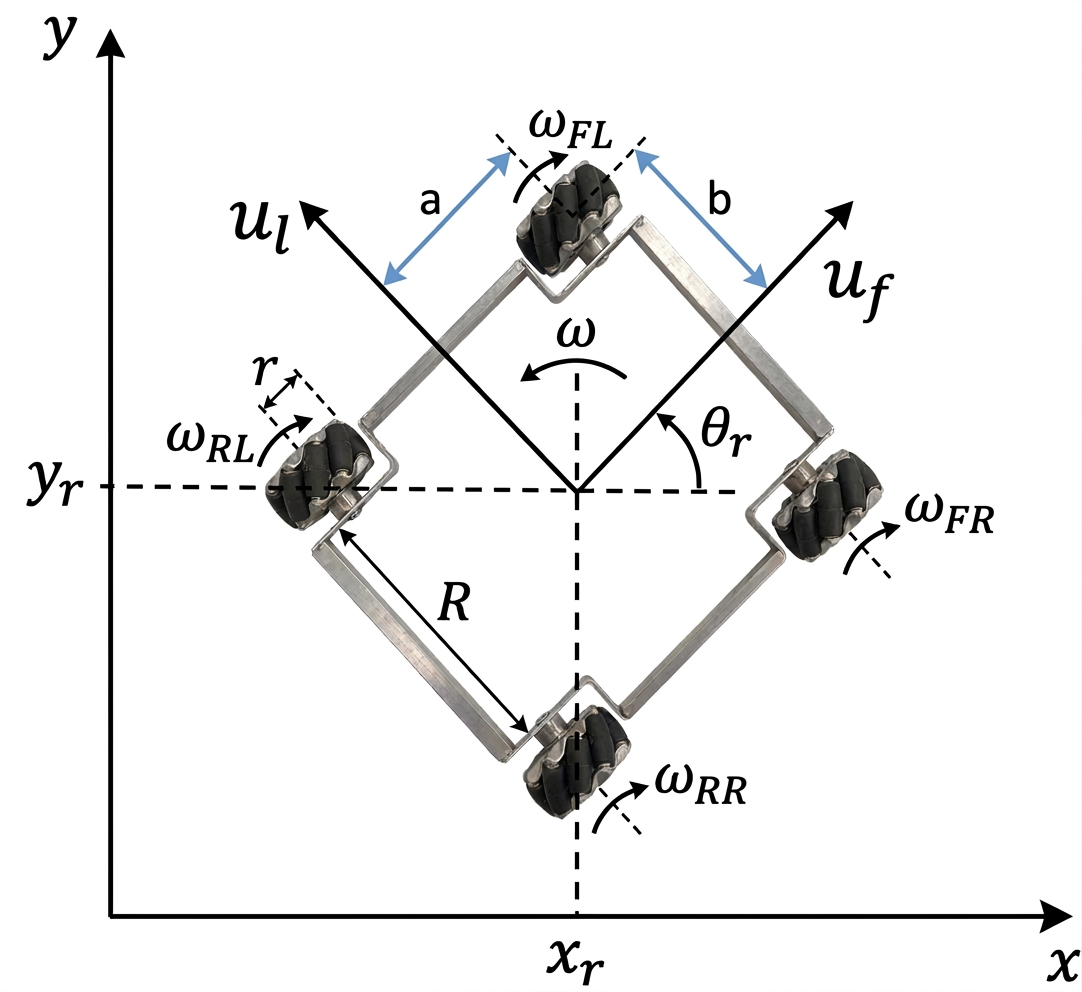
\includegraphics[width=0.5\textwidth]{images/Ch2/Kinematic model mecanum wheels.jpg}
    \caption{Kinematic parameters of a 4-wheel Mecanum drive robot. The distances $a$ and $b$ represent the longitudinal and lateral offsets of the wheels relative to the geometric center (Image adapted from Reque et al. \cite{reque_mechatronics_2021}).}
    \label{fig:mecanum_model}
\end{figure}

\subsection{Direct and Inverse Kinematics}
\label{subsec:holon direct and invecers kin}

Following the kinematic derivations proposed by Taheri et al. \cite{taheri_kinematic_2015}, the mobility of the robot is analyzed by linking the local velocities of the chassis --- namely the linear velocities $v_x$ (forward), $v_y$ (lateral) and the angular velocity $\omega$ --- to the rotational speeds of the four wheels.

The \emph{Inverse Kinematics} determines the required wheel velocities given a desired robot velocity vector $[v_x, v_y, \omega]^T$ generated by the ROS 2 navigation stack. By projecting the velocity of the robot onto the driving direction of each wheel and accounting for the $45^\circ$ slip angle of the rollers, the inverse kinematics is expressed in matrix form as \cite{taheri_kinematic_2015}:
\begin{equation}
    \begin{bmatrix}
        \omega_{FL} \\ \omega_{FR} \\ \omega_{RL} \\ \omega_{RR}
    \end{bmatrix}
    = \frac{1}{r}
    \begin{bmatrix}
         1 & -1 & -(a + b) \\
         1 &  1 &  (a + b) \\
         1 &  1 & -(a + b) \\
         1 & -1 &  (a + b)
    \end{bmatrix}
    \begin{bmatrix}
        v_x \\ v_y \\ \omega
    \end{bmatrix}
\end{equation}

Conversely, the \emph{Direct Kinematics} (or Forward Kinematics) computes the resulting robot velocity given the angular speeds of the four wheels, which is essential for odometry computation. Using the pseudo-inverse of the kinematic matrix \cite{taheri_kinematic_2015}:
\begin{equation}
    \begin{bmatrix}
        v_x \\ v_y \\ \omega
    \end{bmatrix}
    = \frac{r}{4}
    \begin{bmatrix}
         1 &  1 &  1 &  1 \\
        -1 &  1 &  1 & -1 \\
        -\frac{1}{a+b} & \frac{1}{a+b} & -\frac{1}{a+b} & \frac{1}{a+b}
    \end{bmatrix}
    \begin{bmatrix}
        \omega_{FL} \\ \omega_{FR} \\ \omega_{RL} \\ \omega_{RR}
    \end{bmatrix}
\end{equation}

\subsection{Holonomic Mobility and Constraints}
\label{subsec:holonomic_mobility}
As demonstrated by the direct kinematics matrix, the velocity vector $[v_x, v_y, \omega]^T$ can assume any arbitrary value. This mathematically proves that all 3 spatial degrees of freedom can be actuated independently and simultaneously.

To maintain formal symmetry with the differential drive analysis, the mobility of the OmniBase must be evaluated using the same Pfaffian constraint approach. For the PMB2 base, the inability to move laterally resulted in a constraint matrix $A(q)$ of rank 1. Conversely, the OmniBase imposes no differential constraints that cannot be integrated. Consequently, applying the formal approach introduced in Section 2.2.3, the associated Pfaffian constraint equation $A(q)\dot{q} = 0$ is characterized by a null constraint matrix $A(q)$:
\begin{equation}
    \begin{bmatrix} 0 & 0 & 0 \end{bmatrix} 
    \begin{bmatrix} \dot{x} \\ \dot{y} \\ \dot{\theta} \end{bmatrix} = 0
\end{equation}

Because the rank of the constraint matrix is strictly zero, the robot's degree of mobility ($\delta_M$) is exactly equal to the dimension of its planar configuration space ($\delta_M = 3$). The platform is fully holonomic. 

The ability to command a non-zero lateral velocity ($v_y \neq 0$), commonly known as \emph{strafing}, fundamentally alters how path planning algorithms compute trajectories. As noted by PAL Robotics \cite{pal_blog_omni_diff}, this holonomic capability eliminates the need for prior in-place rotations. It allows for smooth, continuous, obstacle-avoiding maneuvers in extremely confined spaces, enabling the robot to maintain a fixed sensory viewpoint (e.g., keeping a camera pointed at a target) while translating seamlessly around it.




\section{Probabilistic Motion Models}
\label{sec:probabilistic_motion_models}

The kinematic formulations derived in the preceding sections provide a deterministic framework for mapping control inputs to the ideal velocities of both the differential and holonomic mobile bases. However, executing navigation tasks in physical or high-fidelity simulated environments introduces a profound divergence between ideal kinematic predictions and actual robot trajectories. To bridge this gap, the deterministic perspective must be replaced by a probabilistic approach that explicitly models the inherent stochasticity of physical interactions. This section establishes the theoretical foundations of probabilistic motion models, transitioning from general actuation uncertainty to the specific odometric noise profiles that characterize the PMB2 and OmniBase platforms.

\subsection{Introduction to Odometry-Based Motion Models}
\label{subsec:intro_odometry_models}
The kinematic models previously analyzed rely on the ideal assumption of pure rolling and no slipping. In real-world applications, however, a mobile robot can never be tracked perfectly through the simple integration of its kinematic equations over time—a practice traditionally known as dead reckoning. The execution of a control command at any given time step $t$ is invariably affected by structural, mechanical, and environmental disturbances, such as wheel slippage, limited encoder resolution, and floor irregularities. 

To robustly navigate under these uncontrollable factors, modern robotics shifts from deterministic kinematics to a probabilistic approach, formalized by Thrun et al. \cite{thrun_probabilistic_2005}. Within this framework, the motion of the robot is modeled as a conditional probability density function (PDF), known as the \emph{motion model}:
\begin{equation}
    p(q_t \mid u_t, q_{t-1}),
\end{equation}
where $q_t$ and $q_{t-1}$ represent the current and previous global poses of the robot in its configuration space, respectively, and $u_t$ denotes the motion input.

In practical autonomous navigation frameworks like ROS 2, the motion input $u_t$ utilized by state estimation and localization algorithms (such as the Adaptive Monte Carlo Localization, or AMCL) is typically not the commanded velocity vector, but rather the \emph{odometry reading} obtained from the wheel encoders. As noted by Thrun et al. \cite{thrun_probabilistic_2005}, odometry-based motion models are generally superior to velocity-based models because encoders directly measure the actual wheel revolutions. This allows the system to inherently capture some of the mechanical discrepancies and actual displacements that a pure software velocity command would completely miss.

The underlying sources of this odometric uncertainty can be classified into systematic and non-systematic errors \cite{thrun_probabilistic_2005}. Systematic errors stem from physical imperfections of the platform, such as unequal wheel diameters or structural misalignments, which introduce a deterministic drift that accumulates predictably. Non-systematic errors, conversely, are entirely stochastic and originate from unpredictable dynamic interactions, including wheel slippage on low-friction surfaces or structural vibrations. 

While odometry provides highly accurate relative displacement data over short intervals, the continuous integration of both systematic and non-systematic errors inevitably leads to unbounded \emph{dead-reckoning drift}. The critical aspect of this work is that the mathematical structure and spatial propagation of this probabilistic noise are strictly dictated by the robot's kinematics. This structural divergence establishes a fundamentally different error accumulation profile between the differential PMB2 and the holonomic OmniBase.

\subsection{Differential Drive Uncertainty (PMB2)}
\label{subsec:differential_uncertainty}
The estimation of odometric uncertainty for the non-holonomic TIAGo PMB2 base is modeled by decomposing the relative movement between two consecutive global poses, $q_{t-1}$ and $q_t$, into three sequential stochastically independent maneuvers (Figure~\ref{fig:thrun_decomposition}): an initial rotation ($\delta_{\text{rot1}}$), a translation ($\delta_{\text{trans}}$), and a final corrective rotation ($\delta_{\text{rot2}}$) \cite{thrun_probabilistic_2005}.

In real-world operations, the actual execution of these components diverges from the nominal encoder readings due to mechanical and environmental disturbances. Following the probabilistic framework established by Thrun et al. \cite{thrun_probabilistic_2005}, the variances ($\sigma^2$) of these error distributions are structurally coupled to the magnitude of the commanded motion parameters through four platform-specific noise coefficients, $\alpha_1, \alpha_2, \alpha_3,$ and $\alpha_4$:
\begin{align}
    \sigma^2_{\text{rot1}} &= \alpha_1 \delta^2_{\text{rot1}} + \alpha_2 \delta^2_{\text{trans}}, \\
    \sigma^2_{\text{trans}} &= \alpha_3 \delta^2_{\text{trans}} + \alpha_4 \left( \delta^2_{\text{rot1}} + \delta^2_{\text{rot2}} \right), \\
    \sigma^2_{\text{rot2}} &= \alpha_1 \delta^2_{\text{rot2}} + \alpha_2 \delta^2_{\text{trans}}.
\end{align}

\begin{figure}[htbp]
    \centering
    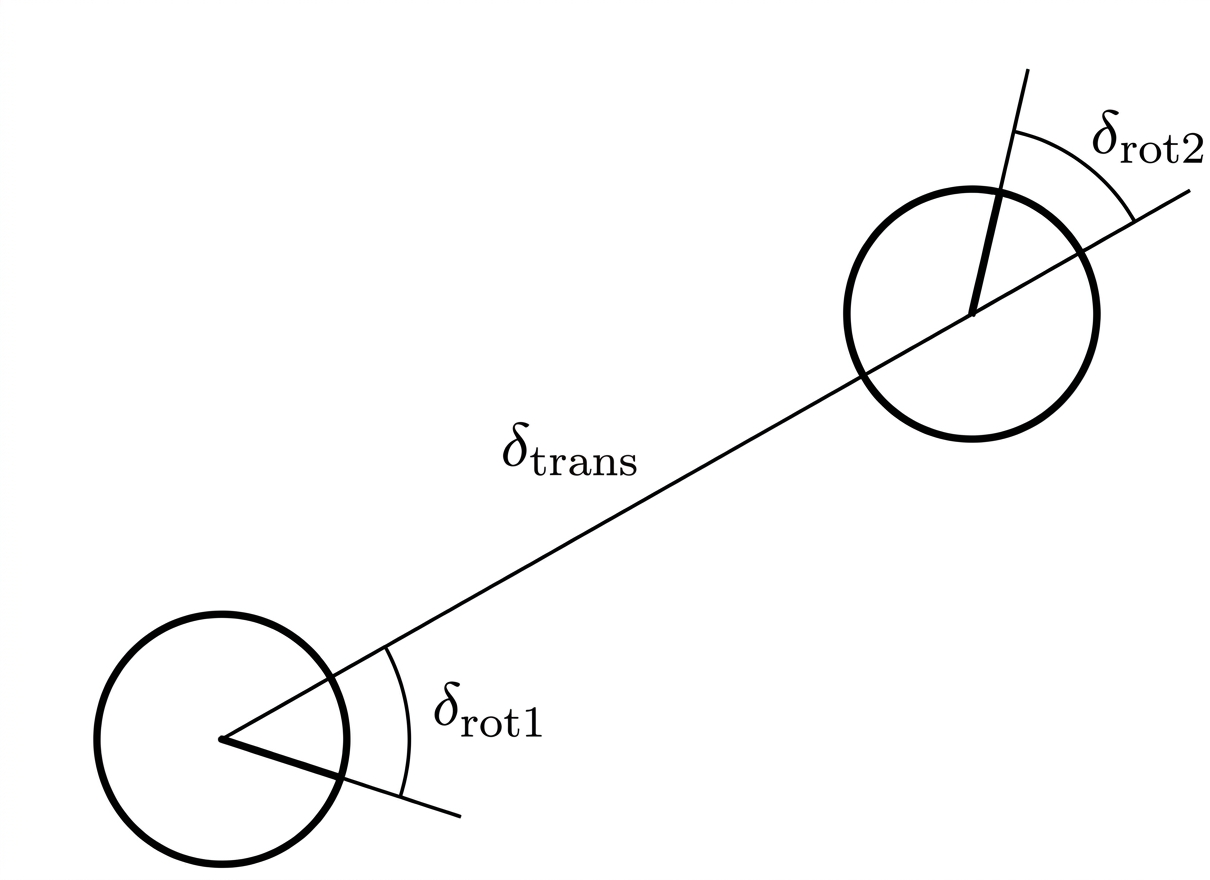
\includegraphics[width=0.5\textwidth]{images/Ch2/Spostamento in tre fasi.jpg}
    \caption{Decomposition of the relative movement between two consecutive poses into an initial rotation, a straight-line translation, and a final corrective rotation (Image adapted from \cite{thrun_probabilistic_2005}).}
    \label{fig:thrun_decomposition}
\end{figure}

For the PMB2 platform, the non-holonomic constraint formulated in Equation~(2.5) dictates that the local lateral velocity must strictly satisfy $v_y = 0$. Consequently, no instantaneous lateral drift can be directly generated within the robot's local frame. Instead, the characteristic "banana-shaped" uncertainty profile (Figure~\ref{fig:banana_shape}) arises because early orientation errors ($\sigma^2_{\text{rot1}}$), caused by wheel micro-slippage or encoder resolution limits during rotation, are geometrically amplified by the subsequent longitudinal translation $\delta_{\text{trans}}$ \cite{thrun_probabilistic_2005}.

\begin{figure}[htbp]
    \centering
    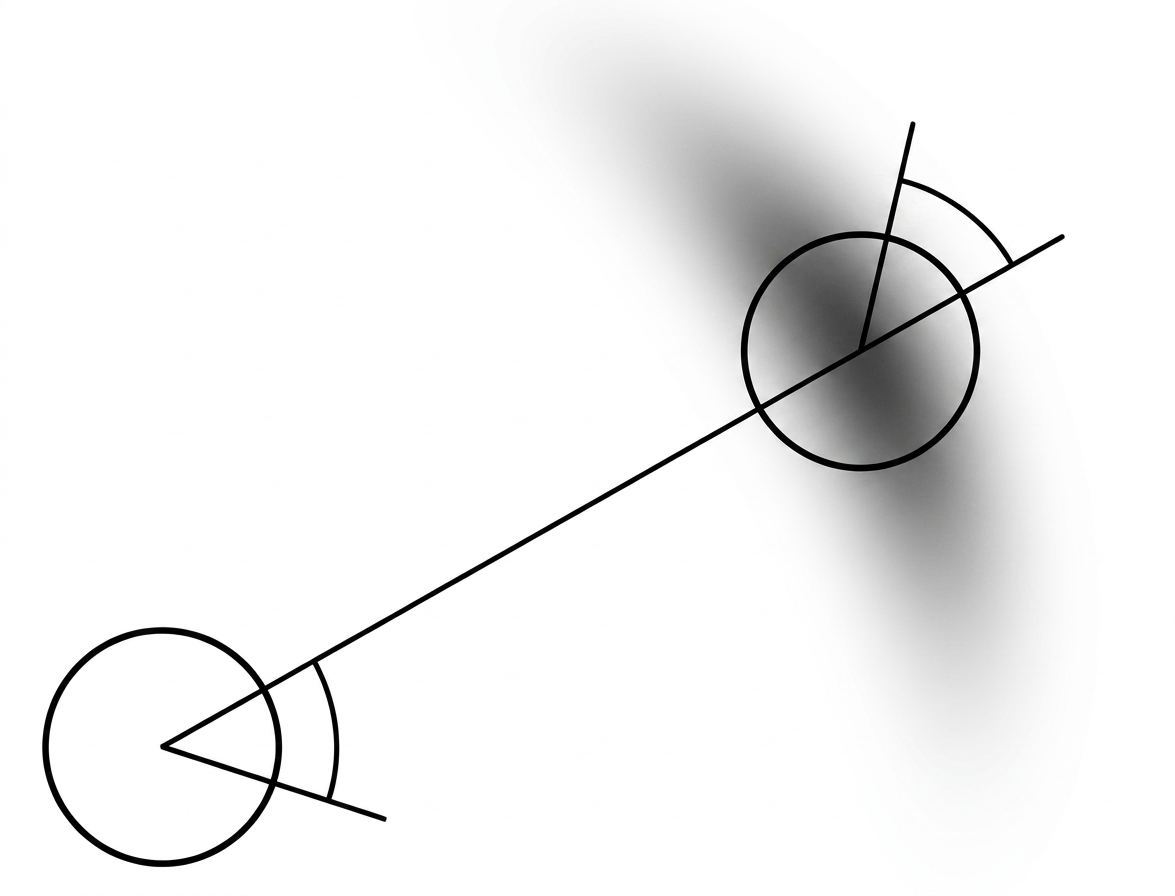
\includegraphics[width=0.5\textwidth]{images/Ch2/Banana shape distribution.jpg}
    \caption{Characteristic "banana-shaped" probability distribution of a differential drive robot. The geometric profile results from early rotational uncertainties being amplified by the subsequent forward translation (Image adapted from \cite{thrun_probabilistic_2005}).}
    \label{fig:banana_shape}
\end{figure}

This makes the bounding of angular variance a critical requirement for the localization stack during forward navigation.


\subsection{Holonomic Drive Uncertainty (OmniBase)}
\label{subsec:holonomic_uncertainty}
In stark contrast to the differential drive, the TIAGo OmniBase utilizes four Mecanum wheels to achieve full holonomic mobility. The fundamental mechanical principle of these wheels relies on passive rollers mounted at a $45^{\circ}$ angle (Figure~\ref{fig:mecanum_forces}). While this design enables instantaneous translations in any planar direction, it purposefully induces continuous, controlled slippage during navigation. 

\begin{figure}[H]
    \centering
    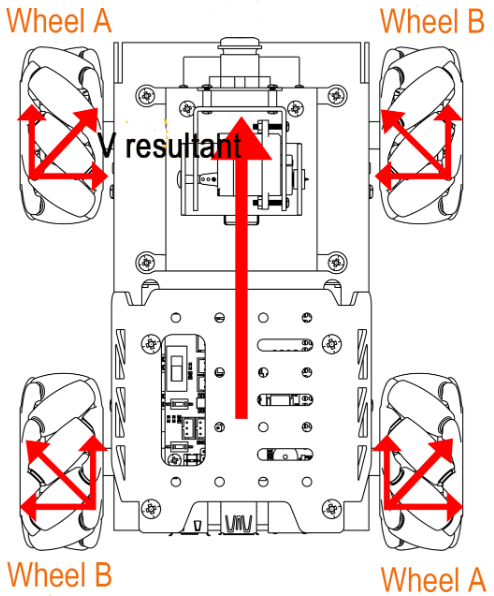
\includegraphics[width=0.40\textwidth]{images/Ch2/Forze risultanti mecanum.png}
    \caption{Kinematic force vectors acting on a Mecanum wheel, illustrating the $45^{\circ}$ orientation of the passive rollers responsible for controlled, multi-directional slippage (Image adapted from \cite{hiwonder_mecanum_2026}).}
    \label{fig:mecanum_forces}
\end{figure}

From a probabilistic perspective, as discussed by Thrun et al. \cite{thrun_probabilistic_2005}, this physical characteristic significantly alters the odometric noise distribution. Unlike the PMB2, the OmniBase is not subject to the non-holonomic lateral constraint ($v_y = 0$). Therefore, the standard unicycle decomposition ($\delta_{\text{rot1}}, \delta_{\text{trans}}, \delta_{\text{rot2}}$) is geometrically inadequate. For a holonomic platform, the relative odometric displacement between two consecutive poses, $q_{t-1}$ and $q_t$, is directly extracted in the robot's local frame as a generic translation along the longitudinal axis ($\delta_x$), a translation along the lateral axis ($\delta_y$), and a rotation ($\delta_\theta$).

Because lateral displacements are both intentionally commanded and inherently affected by the stochastic slippage of the passive rollers, the error propagates simultaneously and is highly coupled across all Cartesian axes. Analogously to the differential model, the variances ($\sigma^2$) for the holonomic drive can be explicitly formulated by mapping the commanded local displacements to the error distributions via a new set of specific noise coefficients, $\alpha_1$ through $\alpha_9$:
\begin{align}
    \sigma^2_{x} &= \alpha_1 \delta_x^2 + \alpha_2 \delta_y^2 + \alpha_3 \delta_\theta^2, \\
    \sigma^2_{y} &= \alpha_4 \delta_x^2 + \alpha_5 \delta_y^2 + \alpha_6 \delta_\theta^2, \\
    \sigma^2_{\theta} &= \alpha_7 \delta_x^2 + \alpha_8 \delta_y^2 + \alpha_9 \delta_\theta^2.
\end{align}

\begin{figure}[H]
    \centering
    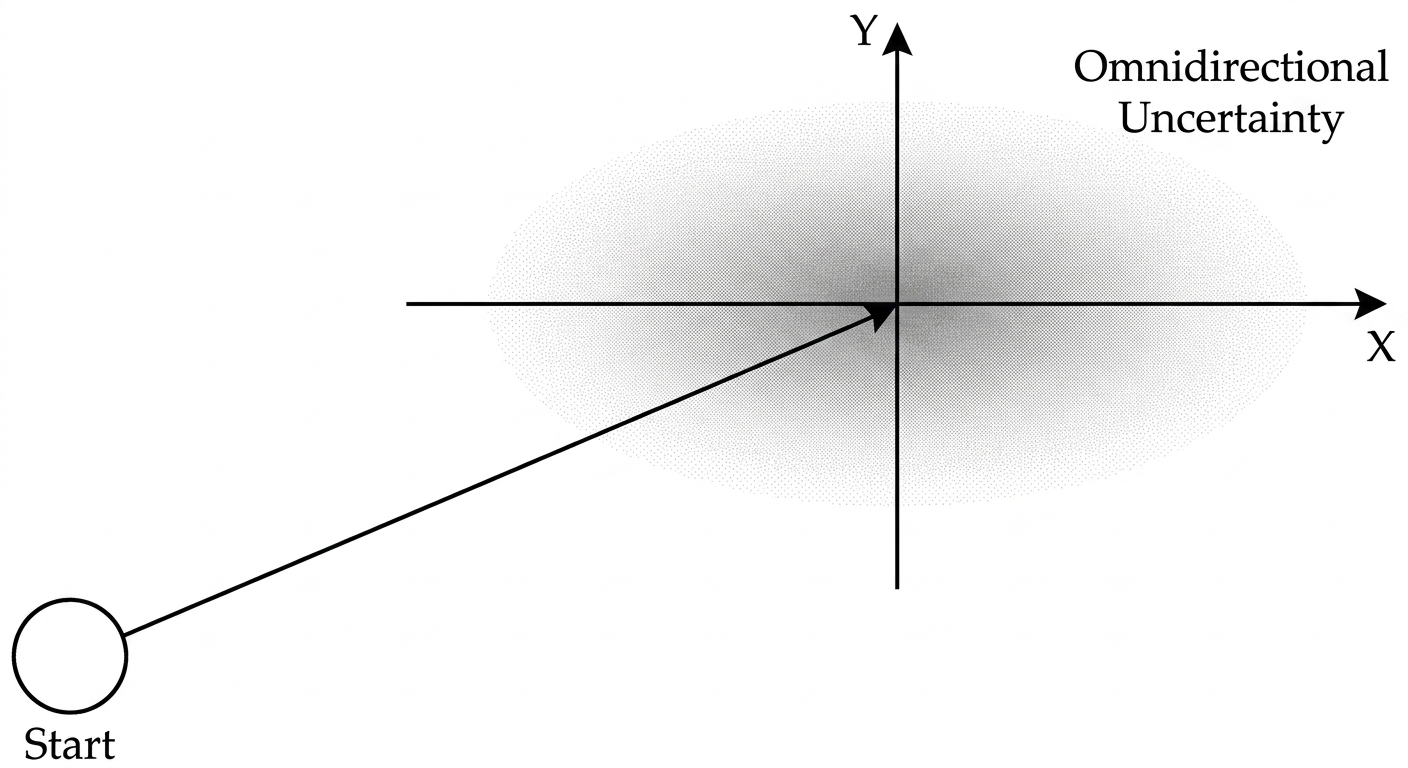
\includegraphics[width=0.7\textwidth]{images/Ch2/cloud shape distribution.jpg}
    \caption{Characteristic probability cloud of an omnidirectional drive. The unconstrained lateral slippage generates a broad uncertainty distribution across all axes, contrasting with the differential "banana-shape".}
    \label{fig:cloud_shape}
\end{figure}

This mathematical formulation clearly demonstrates that the lateral variance $\sigma^2_{y}$ is no longer bounded or negligible. The cross-coupling terms (for example, the influence of the lateral motion $\delta_y$ on the rotational error $\sigma^2_\theta$) dictate that the resulting uncertainty profile expands into a broader, omnidirectional probability cloud (Figure~\ref{fig:cloud_shape}), rather than a tightly constrained curve. This structural variance necessitates more frequent and robust sensory updates from the Nav2 localization stack to prevent rapid dead-reckoning drift during complex holonomic maneuvers.

In practice, the ROS~2 Nav2 framework does not implement this full
nine-coefficient covariance: its \texttt{nav2\_amcl::OmniMotionModel} adopts
a reduced five-parameter form, whose rationale and parameterisation are
detailed in Section \ref{subsec:amcl_tuning}.


\subsection{Comparative Odometry Noise Profile}
\label{subsec:comparative_noise_profile}
The structural and kinematic divergence between the differential PMB2 and the holonomic OmniBase establishes a fundamental trade-off between vehicular mobility and odometric reliability. A systematic comparison of their probabilistic motion models reveals distinct error propagation behaviors that directly influence state estimation.

The non-holonomic PMB2 base features a tightly constrained noise profile. Because it satisfies the zero lateral velocity constraint ($v_y = 0$), the instantaneous generation of lateral drift within the local frame is physically restricted. The odometric uncertainty is primarily driven by rotational noise, which geometrically expands into the characteristic banana-shaped distribution along the transverse axis during forward translation \cite{thrun_probabilistic_2005}. This localized error accumulation allows localization algorithms, such as AMCL within the Nav2 stack, to predict and bound the position variance effectively using highly directional sensory updates.

Conversely, the holonomic OmniBase exhibits a continuous, omnidirectional error propagation. The absence of the lateral velocity constraint enables full planar maneuverability but introduces a highly coupled noise distribution across the $X$, $Y$, and $\theta$ axes simultaneously. This is a direct consequence of the continuous, unmodeled slippage generated by the $45^{\circ}$ passive rollers inherent to the Mecanum wheel design. The resulting uncertainty expands as a broad omnidirectional probability cloud rather than a constrained curve, necessitating more frequent sensor fusion updates to counteract rapid dead-reckoning drift. Consequently, tuning the probabilistic motion parameters within ROS~2 requires the introduction of an additional noise coefficient (the lateral term $\alpha_5$), absent in the differential model, to bound the extra lateral slippage variance and prevent filter divergence during complex, multidirectional maneuvers; the four differential coefficients $\alpha_1$--$\alpha_4$ are themselves kept identical across both platforms.

